\section{Background}

\subsection{Focus on two methods}

In this paper, we focus on two methods for approximating the value of $\pi$. 
The first by French mathematician François Viète, and another discovered by Madhava of Sangamagrama. Two methods with different 
approaches have been chosen for comparison and the process for original discovery of these methods
will be explained. The two in question are one based on 
the infinite series definition of an inverse trigonometric function discovered by Madhava
and one where the value is derived using geometry, by mathematician 
Viète. These two mathematical methods were chosen as they are both 
represent a first occurrence in mathematics: Madhava was the first to 
find the infinite series expansion of the inverse tangent function and Viète was 
the first mathematician to use an infinite product in calculation. 


\subsubsection{An analytical method: Madhava's method}

Madhava is the first mathematician known to have found the series notation for 
the inverse tangent function, in the Kerala school of mathematics of Medieval India 
\cite{amermathmonthly}. The research made at the Kerala school was documented by 
many mathematicians of their time, namely the astronomer-mathematician Jyesthadeva 
in his treatise \textit{Yukti-Bhasa} written in the Malayalam language \cite{oconnor_robertson_2000}. 
Madhava's infinite series expansion of the inverse tangent function can also be 
found in this treatise. R. C. Gupta, in his translation, describes this expansion as one 
where the arc $\theta$ is equal to the sum of a first term, "the product of the given sine 
and radius of the desired arc divided by the cosine of the arc"\footnotemark, followed by terms that "are 
obtained by a process of iteration": in which the original term is multiplied by the 
square of the sine and divided by the square of the cosine. Thereafter, each term is 
divided by an odd number in order (1, 3, 5, 7, \dots). It is then said that the arc can 
be found by "adding and subtracting respectively the terms of odd rank and those of even rank",  
definition of an alternating series. \cite{rc_gupta_mgseries}

\footnotetext{Note: the old Indian meaning for the sine of $\theta$ is $r \sin{\theta}$, where $r$ is the radius. The same applies for the cosine.} 


This text explains what can be written in modern mathematical terms as such:

$r \theta = \frac{r (r \sin{\theta})}{1 (r \cos{\theta})} - \frac{r (r \sin{\theta})^3}{3 (r \cos{\theta})^3} + \frac{r (r \sin{\theta})^5}{5 (r \cos{\theta})^5} - \frac{r (r \sin{\theta})^7}{7 (r \cos{\theta})^7} + \dots$

And for a circle of radius $r = 1$, we can cancel all $r$ terms:

$\theta = \frac{\sin{\theta}}{\cos{\theta}} - \frac{\sin^3{\theta}}{3 \cos^3{\theta}} + \frac{\sin^5{\theta}}{5 \cos^5{\theta}} - \frac{\sin^7{\theta}}{7 \cos^7{\theta}} + \dots$

And because $\frac{\sin{\theta}}{\cos{\theta}} = \tan{\theta}$, the aforementioned expression 
can be simplified to: 

$\theta = \tan{\theta} - \frac{\tan^3{\theta}}{3} + \frac{\tan^5{\theta}}{5} - \frac{\tan^7{\theta}}{7} + \dots$

So then, if we let $\tan{\theta} = \alpha$, we can find the infinite series expansion 
of the arctangent function. 

$\arctan{\alpha} = \alpha - \frac{\alpha^3}{3} + \frac{\alpha^5}{5} - \frac{\alpha^7}{7} + \dots = \theta$

\textit{Yukti-Bhasa} also describes two methods for the calculation of $\pi$. Firstly, 
Madhava's infinite series expansion for $\pi$ is described, which he obtained through 
the previous expansion for the arctangent function. And since $\arctan{1} = \frac{\pi}{4}$,
it can be said that: 

$\frac{\pi}{4} = \arctan{1} = 1 - \frac{1}{3} + \frac{1}{5} - \frac{1}{7} + \dots + \frac{(-1)^n}{2n +1}$

Which in form of an infinite sum can be expressed as: 

$\frac{\pi}{4} = \sum\limits_{n=0}^\infty \frac{(-1)^n}{2n +1}$

Which has come to be known as the Leibniz formula for $\pi$, after the German mathematician 
who discovered the same formula two decades later. \cite{edwards_1994} This series converges to $\pi$, as seen in (Figure 1) \ref{fig:numberline}


However, the method with a faster convergence can be found in a further commentary describing the findings of Madhava that states  
a method for the calculation of the circumference $c$ of a circle of diameter $d$ exists. 
The passage in question from the commentary \textit{Tantrasamgraha-vyakhya} of 
anonymous authorship states that, by following the same argument as stated before, one 
can find the circumference of a circle through a similar infinite sum. The first 
term of this sum would be "the square root of the square of the diameter multiplied by 
twelve", followed by the first term "divided by three in each successive case", and 
when these "are divided in order by the odd numbers, beginning with 1", and after the 
even terms are subtracted from sum of the odd", one is left with the circumference of the 
circle (translation from C. K. Raju). \cite{raju_2007} 

This can be expressed in mathematical terms as such, where we let $c$ be the circumference of 
a circle of diameter $d$: 

$c = \sqrt{12 d^2} - \frac{\sqrt{12 d^2}}{3 \cdot 3} + \frac{\sqrt{12 d^2}}{3^2 \cdot 5} - \frac{\sqrt{12 d^2}}{3^3 \cdot 7} + \dots$

And since $c = \pi d$, for a circle of diameter 1, $c = \pi$, all $d$ terms cancel and 
the expression can be factorized as: 

$c = \pi = \sqrt{12} ( 1 - \frac{1}{3 \cdot 3} + \frac{1}{3^2 \cdot 5} - \frac{1}{3^3 \cdot 7} + \dots )$

Or as an infinite sum:

$\pi = \sqrt{12} \sum\limits_{n=0}^\infty \frac{(-3)^{-n}}{2n+1}$

\subsubsection{A geometric method: Viète's method}

François Viète approached the value of $\pi$ from a 
geometric standpoint, and found an infinite product. 
He was able to calculate $\pi$ to a place of 9 decimal points, in 
the year 1593 \cite{Kreminski}, using his method. His method is reminiscent 
of Archimedes' method, where the length of a side is calculated \cite{archimedespi}, 
but differs in that it consists of finding the area of a polygon of $n$ sides in a circle of constant 
radius, rather than the circumference. As the value of $n$ is increased, the area of the $n$-gon 
tends toward the area of a circle. The geometric origin of this formula 
can be found using simple right-angle trigonometry, by first finding 
the lengths $OH$ and subsequently $BD$ in (Figure 2) \ref{fig:image1}.

\begin{figure}[H]
  \definecolor{qqwuqq}{rgb}{0,0.39215686274509803,0}
  \definecolor{aazzee}{rgb}{0.898039215686, 0.364705882353, 0.294117647059}
  \definecolor{uuuuuu}{rgb}{0.26666666666666666,0.26666666666666666,0.26666666666666666}
  \definecolor{xdxdff}{rgb}{0.49019607843137253,0.49019607843137253,1}
  \definecolor{qqqqzz}{rgb}{0,0,0.6}
  \begin{tikzpicture}[line cap=round,line join=round,>=triangle 45,x=1cm,y=1cm,scale=0.7]
  \clip(-8.372520930232552,-8.50470697674418) rectangle (7.69259534883721,7.028316279069767);
  \draw [shift={(-0.03355999206952884,0)},line width=1pt,color=qqwuqq,fill=qqwuqq,fill opacity=0.10000000149011612] (0,0) -- (0:1.3302325581395344) arc (0:44.77428433325932:1.3302325581395344) -- cycle;
  \draw [line width=0.8pt,color=qqqqzz] (0,0) circle (6cm);
  \draw [line width=1pt, color=aazzee] (4.242640687119286,4.242640687119285)-- (6,0);
  \draw [line width=1pt, color=aazzee] (6,0)-- (4.242640687119286,-4.242640687119285);
  \draw [line width=1pt, color=qqwuqq] (4.242640687119286,-4.242640687119285)-- (4.242640687119286,4.242640687119285);
  \draw [line width=1pt] (-6,0)-- (6,0);
  \draw [line width=1pt] (-4.275936263984878,-4.209081736713964)-- (4.242640687119286,4.242640687119285);
  \draw [line width=1pt] (-4.242640687119285,4.242640687119286)-- (4.242640687119286,-4.242640687119285);
  \draw [line width=1pt] (-0.03355999206952884,0)-- (5.121320343559643,2.1213203435596424);
  \draw [line width=1pt, color=qqwuqq] (-4.242640687119285,4.242640687119286)-- (-4.275936263984878,-4.209081736713964);

  \draw [line width=1pt, dotted, color=aazzee] (0,6)-- (4.242640687119286,4.242640687119285);
  \draw [line width=1pt, dotted, color=aazzee] (0,6)-- (-4.242640687119286,4.242640687119285);

  \draw [line width=1pt, dotted, color=aazzee] (-6,0)-- (-4.242640687119286,4.242640687119285);
  \draw [line width=1pt, dotted, color=aazzee] (-6,0)-- (-4.242640687119286,-4.242640687119285);

  \draw [line width=1pt, dotted, color=aazzee] (0,-6)-- (-4.242640687119286,-4.242640687119285);
  \draw [line width=1pt, dotted, color=aazzee] (0,-6)-- (4.242640687119286,-4.242640687119285);

  \draw [line width=1pt, dotted, color=qqwuqq] (-4.242640687119286,-4.242640687119285)-- (4.242640687119286,-4.242640687119285); 
  \draw [line width=1pt, dotted, color=qqwuqq] (-4.242640687119286,4.242640687119285)-- (4.242640687119286,4.242640687119285); 


  \begin{scriptsize}
  \draw [fill=xdxdff] (4.242640687119286,4.242640687119285) circle (2.5pt);
  \draw[color=xdxdff] (4.4772465116279085,4.623665116279071) node {$B$};
  \draw [fill=xdxdff] (-4.242640687119285,4.242640687119286) circle (2.5pt);
  \draw[color=xdxdff] (-4.295311627906972,4.623665116279071) node {$A$};
  \draw [fill=xdxdff] (-4.275936263984878,-4.209081736713964) circle (2.5pt);
  \draw[color=xdxdff] (-4.336241860465112,-4.55) node {$C$};
  \draw [fill=xdxdff] (6,0) circle (2.5pt);
  \draw[color=xdxdff] (6.237246511627907,0.3873860465116302) node {$E$};
  \draw [fill=xdxdff] (4.242640687119286,-4.242640687119285) circle (2.5pt);
  \draw[color=xdxdff] (4.3772465116279085,-4.5) node {$D$};
  \draw[color=black] (5.3595720930232575,2.3111069767441874) node {$H'$};
  \draw [fill=xdxdff] (5.12,2.12) circle (2.5pt);
  \draw[color=black] (3.947479069767444,-0.615404651162788) node {$H$};
  \draw [fill=xdxdff] (4.242640687119286,0) circle (2.5pt);
  \draw [fill=xdxdff] (0,0) circle (2.5pt);
  \draw[color=uuuuuu] (0.00003720930232879,-0.3464558139534907) node {$O$};
  \draw[color=qqwuqq] (1.5325953488372117,0.3873860465116302) node {$\alpha$};
  \end{scriptsize}
  \end{tikzpicture}
  \label{fig:image1}
  \caption[]{Circle with 1 segment from a $n$-gon with point $H$ and 2 
  segments from an $2n$-gon, one of which on point $H'$, inscribed in 
  a circle of radius $OB$, adapted from (Boris Gourévitch) \cite{borisgourevitch2013}}
  \end{figure}
  
% $$\pi = \frac{2}{\prod_{k = 0}^{\infty} U_{k}}$$    symbolic
With the radius of the circle with center $R = OB$,

$OH = R \cos{\alpha}$ 

and

$BD = 2BH = 2 R \sin{\alpha}$

Since the equation for the area of a polygon is defined as $A = \frac{p \cdot a}{2}$, 
where $p$ is the perimeter of the polygon and $a$ is the apothem, in this case $BD \cdot n$ 
and $OH$ respectively, let $A_{n}$ equal the area of 
the polygon with $n$ sides such that: \\
$A_{n} = \frac{OH \cdot BD \cdot n}{2}$ \\
$A_{n} = \frac{R \cos{\alpha} \cdot 2 R \sin{\alpha} \cdot n}{2} = n R^2 \sin{\alpha} \cos{\alpha}$

And if n is multiplied by 2, the angle $\angle \alpha$ is divided by 2, 
and the new area becomes: 

$A_{2n} = 2n R^2 \sin{\frac{\alpha}{2}} \cos{\frac{\alpha}{2}}$

So it can be written that, by definition, the ratio of 
the area of an $n$-gon to one of a $2n$-gon is

$\frac{A_{n}}{A_{2n}} = \frac{n R^2 \sin{\alpha} \cos{\alpha}}{2 n R^2 \sin{\frac{\alpha}{2}} \cos{\frac{\alpha}{2}}} = \frac{\sin{2 \alpha}}{2 \sin{\alpha}}$

Which through the trigonometric identity $\sin{2 \theta} = 2\sin{\theta} \cos{\theta}$ can 
be simplified to:

$\frac{A_{n}}{A_{2n}} = \frac{2\sin{\alpha} \cos{\alpha} }{2\sin{\alpha}}  = \cos{\alpha}$

It can be then written that, through a new variable $P$, \\
$P = \frac{A_{n}}{A_{2n}} \frac{A_{2n}}{A_{4n}} \frac{A_{4n}}{A_{8n}} \dots \frac{A_{(k-2)n}}{A_{kn}} \frac{A_{kn}}{A}$ \\
where $A$ is the area of the circle of radius $R$ 
in \ref{fig:image1}. 

So $P = \frac{A_{n}}{A}$, since the values $A_{kn}$ cancel, and 
so it is true that $P = \frac{A_{n}}{A} \Leftrightarrow A = \frac{A_{n}}{P}$. The 
value of $R = 1$ in this case, and since the area of a circle is defined 
by $A = \pi R^2$, therefore: \\
$\pi = \frac{A_{n}}{P}$ \\
By definition, we can say that as the value $k$ approaches infinity, the area of the $kn$-gon 
approaches that of a circle, and therefore, the value of $\pi$.

$\frac{A_{n}}{\cos{\alpha} \cos{\frac{\alpha}{2}} \cos{\frac{\alpha}{4}} \dots}
\to_{k \to \infty} \pi$

Where the value of $A_{n}$ is the area of the first polygon, with $n=4$ sides, and as such 
$A_{n} = 4 \sin{45} \cos{45} = 2$. We can define: \\
$U_{0} = \cos{a} = \cos{45} = \frac{1}{\sqrt{2}}$ \\
$U_{1} = cos{\frac{\alpha}{2}}$ \\
Which we can, through the trigonometric identity 
$\cos^2{\theta} = \frac{1}{2} + \frac{1}{2} \cos{2\theta}$, simplify as
$U_{1} = \sqrt{\frac{1}{2} + \frac{1}{2} U_{0}}$ \\
So it can be said that $U_{n} = \sqrt{\frac{1}{2} + \frac{1}{2} U_{n - 1}}$, which leads to 
a fully defined expression for the value of pi, using an infinite product: 

$\pi = \frac{2}{\prod\limits_{k=0}^\infty U_{k}}, U_{0} = \frac{1}{\sqrt{2}}, U_{n} = \sqrt{\frac{1}{2} + \frac{1}{2} U_{n - 1}}$ \footnotemark

\footnotetext{where $\prod$ signifies a product. Similar expression to $\sum$ }







\begin{figure}[h]

    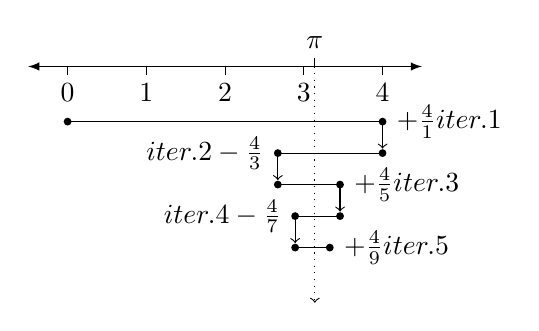
\begin{tikzpicture}
        \draw[latex-latex] (-0.5,0) -- (4.5,0);% the x-axis
        \foreach \x in  {0,...,4} % tick marks
          \draw (\x,0) -- (\x,-3pt);
        \foreach \x in {0,...,4} % the numbers
          \node [below] at (\x,-0.1) {$\x$};
        \node [below] at (3.14,0.5) {$\pi$};
        \draw (3.14,0) -- (3.14,3pt);

        \draw[->, dotted] (3.14,0) -- (3.14,-3);% the x-axis

        \draw[xshift=-1cm] (1,-0.7) node[circle,fill,inner sep=1pt](a){} -- (5,-0.7) 
node[circle,fill,inner sep=1pt,label=right:$+\frac{4}{1} \boxed{\text{ iter. 1}}$](b){};

\draw[xshift=-1cm] (3.67,-1.1) node[circle,fill,inner sep=1pt, label=left:$\boxed{\text{iter. 2 }} -\frac{4}{3}$](c){} -- (5,-1.1) 
node[circle,fill,inner sep=1pt](d){};

\draw[xshift=-1cm] (3.67,-1.5) node[circle,fill,inner sep=1pt](e){} -- (4.46,-1.5) 
node[circle,fill,inner sep=1pt, label=right:$+\frac{4}{5} \boxed{\text{ iter. 3}}$](f){};

\draw[xshift=-1cm] (3.89,-1.9) node[circle,fill,inner sep=1pt, label=left:$\boxed{\text{iter. 4 }} -\frac{4}{7}$](g){} -- (4.46,-1.9) 
node[circle,fill,inner sep=1pt](h){};

\draw[xshift=-1cm] (3.89,-2.3) node[circle,fill,inner sep=1pt](i){} -- (4.33,-2.3) 
node[circle,fill,inner sep=1pt, label=right:$+\frac{4}{9} \boxed{\text{ iter. 5}}$](j){};




\draw[->, to path={-| (\tikztotarget)}]
  (b) edge (d) (c) edge (e) (f) edge (h) (g) edge (i);
     \end{tikzpicture}
    
\label{fig:numberline}
\caption[]{A number line demonstrating the convergence of Madhava's first method for the 
calculation of $\pi$. Adapted from (V. M. Jamkar) \cite{jamkar_2018}}
\end{figure}


